% !TeX root = ../../../book.tex
\subsection{好友倾向}\label{sec:section1.4.4}

\subsubsection*{问题描述}

这个问题源于匈牙利社会学家的一则轶事,以及他对儿童朋友圈的观察。

\begin{quote}
    ``20 世纪 50 年代,匈牙利社会学家 S. Szalai 研究了儿童之间的友谊关系。他观察到,在任何大约 $20$ 个孩子的群体中,总能找到四个孩子,他们彼此都是朋友,或者四个孩子中没有任何两个是朋友。在得出社会学结论前,S. Szalai 咨询了三位著名的匈牙利数学家:Erdős, Turán 和 Sós。经过简短的讨论,他们表明这实际上是一种数学现象,而非社会学现象。对于至少 $18$ 个元素上的任意对称关系 $R$,存在 $4$ 个元素的子集 $S$,使得 $R$ 包含 $S$ 中的所有对,或不包含其中任何对。这一事实是 1930 年证明的拉姆齐定理 (Ramsey's theorem) 的一个特例,它奠定了拉姆齐理论 (Ramsey theory) 的基础,后来发展成为组合数学中的一个丰富领域。''\begin{flushright}——(引自麻省理工学院 Jacob Fox 教授的\href{https://math.mit.edu/~fox/MAT307-lecture01.pdf}{讲义}。)\end{flushright}
\end{quote}

现在,我们沿袭相同思路提出一个类似问题,但使用更小的数字。具体来说,我们想要找出\emph{满足}其中三人互为朋友或敌人的最小群体规模。

\begin{quote}
    假设在一群人中,任意两人要么是朋友,要么是敌人,且没有其他关系(例如没有熟人或亦敌亦友的情况)。尝试为四人群体中的每一对指定朋友或敌人关系,使得不存在三人组彼此都是朋友或全是敌人。五人群体能否实现这一条件?六人呢?七人?十人?二十人?请确定最小的群体规模,使得无论如何指定关系,都\emph{保证}存在一个三人小组,他们要么全是朋友,要么全是敌人。
\end{quote} 

请仔细思考一下,然后再翻页阅读解答。

\clearpage

\subsubsection*{有效地表述问题}

你解出来了吗?这是一个相当棘手的问题,所以即使没有得出答案也无需气馁。事实上,探究问题的过程与找到答案同等重要,因为解决路径多种多样,观察不同人如何理解这个问题总是饶有趣味。

首先,我们探讨如何清晰描述这种情境。针对此类问题,我们需要考虑一个固定规模的人群,并分析其中任意两人之间的关系。为高效验证三人子集是否满足特定性质,即是否存在三人\emph{互为}朋友或\emph{互为}敌人,必须找到一种简洁且易于阐释的关系表示方法。我们将这种三人关系称为``\textbf{同质性}''。

如何实现呢?如何表示人物及其关系?我们可以对人群编号,列出所有数对并标注 $F$(朋友)或 $E$(敌人)。以四人小组为例:
\[12F \qquad 13E \qquad 14F \qquad 23F \qquad 24E \qquad 34F\]

该群体是否满足同质性?直观验证并不容易:编号方式增加了定位三人子集的难度,且需逐一检查所有子集是否形成 $E E E$ 或 $F F F$ 关系。或许在深入解题前,我们应该寻求一种更优的信息呈现方式。能否想出更直观的方法,表示人群中每对个体的朋友或敌人关系?具体来说,我们希望通过高效手段定位三人子集,并快速识别其关系性质。

让我们尝试将每个人表示为一个点,两人间的关系用连线表示——例如蓝线代表朋友,红线代表敌人(注意:每对个体必有且仅有一种关系,故所有点之间均有彩线连接)。下图对应上述关系描述:

\begin{center}
    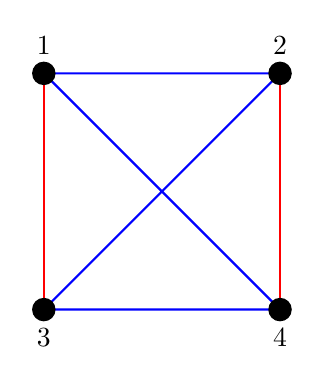
\begin{tikzpicture}[thick,scale=0.5]
        \coordinate (A) at (0,6);
        \coordinate (B) at (6,6);
        \coordinate (C) at (0,0);
        \coordinate (D) at (6,0);
        \draw[blue] (A) node[black, above, yshift=3pt]{$1$}
        -- (B) node[black, above, yshift=3pt]{$2$}
        -- (C) node[black, below, yshift=-3pt]{$3$}
        -- (D) node[black, below, yshift=-3pt]{$4$}
        -- (A);
        \draw[red] (A)--(C);
        \draw[red] (B)--(D);
        \foreach \n in {A,B,C,D}
            \node at (\n)[circle,fill,inner sep=3pt]{};
    \end{tikzpicture}
\end{center}

现在,我们要如何验证同质性?需寻找三个点(三人),其所有连线均为蓝色(全友)或红色(全敌)。这正是寻找\textbf{单色三角形}的过程!(注意:三角形顶点须为原始点,而非连线交点;术语\emph{单色 (monochromatic)} 源于希腊语 \emph{monos} 和 \emph{khroma},分别表示``一个''和``颜色''。)这种表示法更直观且便于快速检验。

根据上图,我们解决了四人问题:存在一种朋友/敌人的特定配置关系,使得其中不存在全友或全敌的三人子集。这表明四人群体可能避免同质性,故无法\emph{保证}四人中必然存在同质子集。

能否构造另一种满足该性质的配置?如何判断其与已有配置\emph{不同}?满足条件的配置共有多少种?现在请尝试构造一个\emph{必然存在}同质三人子集的配置——其形态如何?此类配置又有多少种?

\subsubsection*{重述 $n = 5$ 的问题}

让我们继续思考由五个人组成的小组。我们的图需要调整,因为现在有五个点,这意味着需要绘制更多的线。尽管如此,我们仍会用蓝色或红色线填充所有连线,并确保没有单色三角形。这可能吗?(提示:尝试将点排列成规则五边形,然后填充连线。)尝试几次,看看你的排列是否有效。随机添加几条线,并通过确保新线不会形成单色三角形来指导你的选择,这也可能有帮助。

你做出来了吗?翻页看看我们是如何做的……

\clearpage

\subsubsection*{解答:$n=5$}

这是我们在五个点之间连线的红/蓝线配置,完全避免了同质性:

\begin{center}
    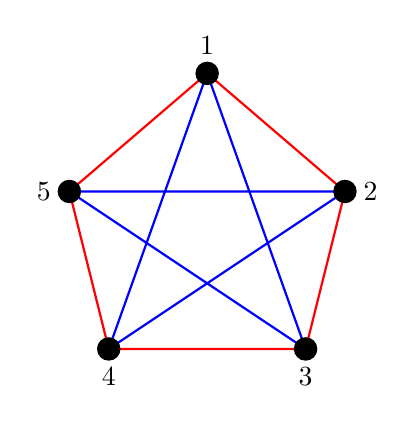
\begin{tikzpicture}[thick,scale=0.5]
        \coordinate (A) at (0,0);
        \coordinate (B) at (5,0);
        \coordinate (C) at (6,4);
        \coordinate (D) at (2.5,7);
        \coordinate (E) at (-1,4);
        \draw[red] (A) node[black, below, yshift=-3pt]{$4$}
        -- (B) node[black, below, yshift=-3pt]{$3$}
        -- (C) node[black, right, xshift=3pt]{$2$}
        -- (D) node[black, above, yshift=3pt]{$1$}
        -- (E) node[black, left, xshift=-3pt]{$5$}
        -- (A);
        \draw[blue] (A)--(D)--(B)--(E)--(C)--(A);
        \foreach \n in {A,B,C,D,E}
            \node at (\n)[circle,fill,inner sep=3pt]{};
    \end{tikzpicture}
\end{center}

请注意该图形优雅的对称性:所有红线均位于五边形的外侧,所有蓝线均位于图形内部。原因是,任意三个相邻点构成的三角形必须使用两条外线和一条内线,而任意三个不相邻点构成的三角形必须使用两条内线和一条外线。(想一想:为什么我们不能用三条内线或三条外线组成一个三角形?)这\emph{保证}了我们构成的任何三角形都会使用两种不同颜色的线,所以这个图形没有单色三角形!当然,我们可以检查图中所有可能的三角形,并确保它们都不是单色的。这样的三角形有多少个?你能多快手工找到所有这些三角形?这样做是否更容易,或者利用我们上面提到的内部/外部属性?

也许你找到的解决方案与我们的图形不同。你怎么知道它是否是不同的图形?你的图中有多少条蓝线、多少条红线?我们的图中呢?尝试通过移动点来重绘图形,但保持点之间的连接关系(即任意两点之间连线的颜色)。你能把你的图形调整得跟我们的一样吗?你认为这对本问题的解的数量意味着什么?

\subsubsection*{$n=6$ 的情况}

现在我们可以思考六个人的情况了。考虑六个点以及它们之间所有可能的连线,我们需要用蓝色或红色为每条线上色,并确保图中不存在所有边颜色相同的三角形。绘制前,请回顾四个点和五个点时我们找到的解决方案。这些解的结构如何?这次我们需要画多少条边?能否尝试构造一个与五点解相似的图形?思考当前问题与先前工作的相似之处往往大有裨益。现在,请尝试画出这个图形并观察结果。

图形是否有效?若无效,问题何在?你在何处遇到了困难?在被迫画出单色三角形之前,最多能添加多少条边?换句话说,在加入下一条必然形成单色三角形(无论颜色)的边之前,图中最多能容纳多少条边?虽然这些问题看似偏离了解决当前难题的主线,但它们本身极具启发性,并可能引导我们找到解法或其推广。为便于说明,下图展示了我们为边分配红蓝两色的一种方案。为何在此处停笔?还需添加多少条边?我们能否继续添加?

\begin{center}
    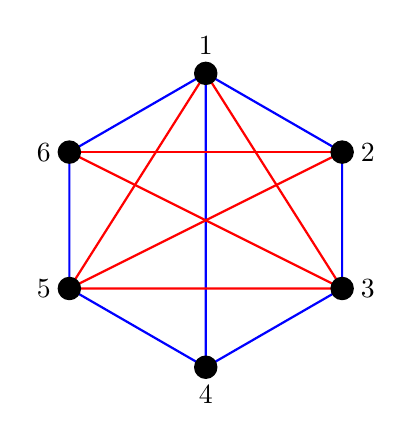
\begin{tikzpicture}[thick,scale=0.5]
        \coordinate (A) at (0,0);
        \coordinate (B) at (-3.4642,2);
        \coordinate (C) at (-3.4642,5.4642);
        \coordinate (D) at (0,7.4642);
        \coordinate (E) at (3.4642,5.4642);
        \coordinate (F) at (3.4642,2);
        \draw[blue] (A) node[black, below, yshift=-3pt]{$4$}
        -- (B) node[black, left, xshift=-3pt]{$5$}
        -- (C) node[black, left, xshift=-3pt]{$6$}
        -- (D) node[black, above, yshift=3pt]{$1$}
        -- (E) node[black, right, xshift=3pt]{$2$}
        -- (F) node[black, right, xshift=3pt]{$3$}
        -- (A)
        -- (D);
        \draw[red] (B)--(E);
        \draw[red] (C)--(F);
        \draw[red] (B)--(D)--(F)--(B);
        \draw[red] (C)--(E);
        \foreach \n in {A,B,C,D,E,F}
            \node at (\n)[circle,fill,inner sep=3pt]{};
    \end{tikzpicture}
\end{center}

我们面临的局面颇具深意,因其性质与先前情况截然相反。在四点与五点情形中,我们试图证明\emph{可以}通过边的着色方案避免单色三角形——只需构造出满足条件的\emph{具体}图形即可证明其存在性。然而对于六个点,似乎无法通过边的着色避免单色三角形。如何证明这一结论?最直接的想法是枚举所有可能的着色方案,并论证每种方案下至少存在一个单色三角形。这可行吗?着色方案共有多少种?如何在给定图形中快速定位单色三角形?回忆我们如何处理五点图形:我们注意到任何三角形必须包含\emph{至少}一条外部边与\emph{至少}一条内部边,这保证了三角形必含两种颜色的边。能否在此采用类似思路,确立某种\emph{必然}导致单色三角形存在的性质?

问题在于,六个点构成的图形中边的着色方案数量过于庞大,难以手动穷尽!图中需着色的边共有 $15$ 条,每条边可选红蓝两色,因此共有 $2^{15}$ 种着色方案——这是一个天文数字!(实际同构类会略少,因为部分方案在某种意义上是等价的;更专业地说,它们是``\emph{同构的}''。)

\subsubsection*{解答:处理\emph{任意}图形}

我们需要更巧妙的方法来论证,以便在不绘制特定图形的情况下证明\emph{任意}图形的性质。也就是说,我们需要找到对所有可能的六点图形都成立的事实,并据此推断出必然存在单色三角形。一种解决思路是关注图形的局部结构。具体而言,任取六个点中的一个,考虑从该点引出的五条边。例如,我们可能得到如下图形:

\begin{center}
    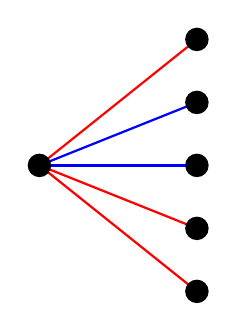
\begin{tikzpicture}[thick,scale=0.2]
        \coordinate (A) at (-6,0);
        \coordinate (B) at (4,4);
        \coordinate (C) at (4,0);
        \coordinate (D) at (4,8);
        \coordinate (E) at (4,-4);
        \coordinate (F) at (4,-8);
        \draw[blue] (A)--(C);
        \draw[blue] (A)--(B);
        \draw[red] (A)--(D);
        \draw[red] (A)--(E);
        \draw[red] (A)--(F);
        \foreach \n in {A,B,C,D,E,F}
            \node at (\n)[circle,fill,inner sep=3pt]{};
    \end{tikzpicture}
\end{center}

有多少条蓝边,多少条红边?这有些棘手:我们并非针对任何\emph{特定}图形(如上图),而是寻求适用于所有可能图形的结论。因此无法给出具体答案。面对一个\textbf{任意}图形,我们必须构建一个普遍有效的论证。

关键点在于:从该点出发的五条边中,必有三条同色(蓝或红)。试想,若非如此,则蓝边不超过两条,红边也不超过两条,总计最多四条边。但实际有五条边!(这是``\emph{抽屉原理}''的典型应用:无法将五个物体按两种颜色分类,而不使某一颜色达到三个。该原理是解决此类问题的有力工具,详见 \ref{sec:section8.6} 节。)

至此,我们得到了什么?从任意一个六点完全图中选定一点,该点必引出三条同色边。颜色可能为红或蓝,因此不能假定仅为红色;若假设为红色进行论证,之后还需讨论蓝色情况。为简化,我们首先分析从该点引出三条红边的情况(暂不限定其他边的颜色):

\begin{center}
    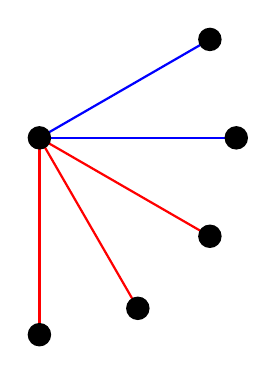
\begin{tikzpicture}[thick,scale=0.5]
        \coordinate (A) at (0,0);
        \coordinate (B) at (4.33,2.5);
        \coordinate (C) at (5,0);
        \coordinate (D) at (4.33,-2.5);
        \coordinate (E) at (2.5,-4.33);
        \coordinate (F) at (0,-5);
        \draw[blue] (A)--(C);
        \draw[blue] (A)--(B);
        \draw[red] (A)--(D);
        \draw[red] (A)--(E);
        \draw[red] (A)--(F);
        \foreach \n in {A,B,C,D,E,F}
            \node at (\n)[circle,fill,inner sep=3pt]{};
    \end{tikzpicture}
\end{center}

现在,如何添加剩余边才能避免三点间出现同色三角形?由于未限定孤立点之间边的颜色,我们聚焦于底部的三个点。它们之间的边可能是什么颜色?若其中任一条为红色,则其两个端点与原始点便构成红色三角形!这就有问题了。

\begin{center}
    \begin{tikzpicture}[thick,scale=0.5]
        \coordinate (A) at (0,0);
        \coordinate (B) at (4.33,2.5);
        \coordinate (C) at (5,0);
        \coordinate (D) at (4.33,-2.5);
        \coordinate (E) at (2.5,-4.33);
        \coordinate (F) at (0,-5);
        \draw[blue] (A)--(C);
        \draw[blue] (A)--(B);
        \draw[red] (A)--(D);
        \draw[red] (A)--(E);
        \draw[red] (A)--(F);
        \draw[red] (E)--(F);
        \draw [red,-stealth,very thick] (-2,-2.4) node[red, above]{$\text{红色三角形}$} -- (1,-3.5);
        \foreach \n in {A,B,C,D,E,F}
            \node at (\n)[circle,fill,inner sep=3pt]{};
    \end{tikzpicture}
\end{center}

避免此情况的唯一方法是将这三条边全染为蓝色。但此时,这三个点之间就形成了蓝色三角形!可见无论如何操作,都无法避免单色三角形!

\begin{center}
    \begin{tikzpicture}[thick,scale=0.5]
        \coordinate (A) at (0,0);
        \coordinate (B) at (4.33,2.5);
        \coordinate (C) at (5,0);
        \coordinate (D) at (4.33,-2.5);
        \coordinate (E) at (2.5,-4.33);
        \coordinate (F) at (0,-5);
        \draw[blue] (A)--(C);
        \draw[blue] (A)--(B);
        \draw[red] (A)--(D);
        \draw[red] (A)--(E);
        \draw[red] (A)--(F);
        \draw[blue] (F)--(D)--(E)--(F);
        \draw [blue,-stealth,very thick] (5.5,-3.8) node[blue, right]{$\text{蓝色三角形}$} -- (2.5,-3.8);
        \foreach \n in {A,B,C,D,E,F}
            \node at (\n)[circle,fill,inner sep=3pt]{};
    \end{tikzpicture}
\end{center}

现在回到抽屉原理的初始结论。若原理保证的三条同色边是蓝色而非红色呢?论证结构完全一致:观察底部三点间的边,

\begin{center}
    \begin{tikzpicture}[thick,scale=0.5]
        {
            \coordinate (A) at (0,0);
            \coordinate (B) at (4.33,2.5);
            \coordinate (C) at (5,0);
            \coordinate (D) at (4.33,-2.5);
            \coordinate (E) at (2.5,-4.33);
            \coordinate (F) at (0,-5);
            \draw[red] (A)--(C);
            \draw[red] (A)--(B);
            \draw[blue] (A)--(D);
            \draw[blue] (A)--(E);
            \draw[blue] (A)--(F);
            \draw[blue] (E)--(F);
            \draw [blue,-stealth,very thick] (-2,-2.4) node[blue, above]{$\text{蓝色三角形}$} -- (1,-3.5);
            \foreach \n in {A,B,C,D,E,F}
                \node at (\n)[circle,fill,inner sep=3pt]{};
        }
        {
            \coordinate (A1) at (8,0);
            \coordinate (B1) at (12.33,2.5);
            \coordinate (C1) at (13,0);
            \coordinate (D1) at (12.33,-2.5);
            \coordinate (E1) at (10.5,-4.33);
            \coordinate (F1) at (8,-5);
            \draw[red] (A1)--(C1);
            \draw[red] (A1)--(B1);
            \draw[blue] (A1)--(D1);
            \draw[blue] (A1)--(E1);
            \draw[blue] (A1)--(F1);
            \draw[red] (F1)--(D1)--(E1)--(F1);
            \draw [red,-stealth,very thick] (13.5,-3.8) node[red, right]{$\text{红色三角形}$} -- (10.5,-3.8);
            \foreach \n in {A1,B1,C1,D1,E1,F1}
                \node at (\n)[circle,fill,inner sep=3pt]{};
        }
    \end{tikzpicture}
\end{center}

若添加任何蓝边,会与原始点形成蓝色三角形;若全染红色,则三点间形成红色三角形!因此,无论最初的三条同色边是红色还是蓝色,论证过程完全\emph{对称}。数学家常利用这种对称性简化证明,表述为``不失一般性,假设三条边为红色''。这意味着,若选择蓝色,后续论证在数学结构上完全相同,故无需重复书写。实际上,这种情况非常常见,以至于``不失一般性''这个术语有时会缩写为 \textbf{WOLOG} 或 \textbf{WLOG} (without loss of generality)。

\subsubsection*{解答:结果总结}

截至目前我们取得了哪些进展?我们绘制了\emph{特定}图形,证明在四个或五个点之间可以着色连线而不形成单色三角形,同时推断\emph{任意}六个点构成的图形\emph{必然}包含单色三角形。对应回原始问题的朋友/敌人表述,这意味着任意六人群体中都存在一个三人组,其成员要么全部互为朋友,要么全部互为敌人。

值得注意的是,将问题转化为点线模型极具启发性;它使我们完全脱离可能分散注意力的社交背景,并简化了术语体系——将人际关系标记简化为两点间的连线。这是极具价值的解题策略:提炼问题的核心结构(底层逻辑、元素间关系及其相互作用),并据此重构表述。这种方法不仅使复杂问题更易于理解和处理,还能指导我们建立更优的符号系统。试想若坚持使用``$13F, 23E, \dots$''这类符号进行推演,也许最终也能求解,但过程必将困难重重!

原题核心目标之一是确定满足特性的最小群体规模。我们是否已完成此目标?六是否为该下界?在任意七人群体中,必然包含六人子群,而前述结论表明该子群中必定存在同质三人组(全友或全敌)。此性质自然推广至更大规模的群体,因此六确实为所求的精确下界。这与匈牙利社会学家在四人子群中观察到的现象类似,而当前问题因规模更大而显著复杂化——我们实际解决的是更小规模的简化案例。两者均属\textbf{拉姆齐理论}范畴,该组合数学与图论分支致力于探寻此类``下界规律'':当结构(如人群)规模增长至临界点时,\emph{必然}出现具备特定性质的子结构(如全友/全敌三人组)。这一始于社会现象的研究,最终被严格证明为数学定理。多么奇妙啊!

\subsubsection*{泛化:留给你的问题}

在继续之前,让我们提出一些有趣且相关的问题。如果我们要寻找不同规模的同质子群(例如四人、五人或十二人)该怎么办?一般来说,我们必须有更多的人才能保证找到这样的子群。我们能否总是这样做?也就是说,给定任何所需的子群大小,我们能否像之前那样确定一个下界?即使没有找到具体的数字,你能想出证明这种下界存在的方法吗?此外,如果我们允许第三种可能性:朋友、敌人或陌生人,又会怎样?我们能否回答关于同质子群的类似问题?这些都与拉姆齐理论相关,其中一些问题非常困难,需要数学家多年努力才能解决。许多看似简单的问题至今仍悬而未决!如果你在这些问题上没有进展,请不要灰心。我们相信,任何尝试和思考都是有意义且有益的。

\subsubsection*{解题心得}

这个问题的解决涉及几个难点。首先,我们必须找到一种方式来有效地解释谜题,以便解决问题,这涉及引入适当的符号来表示元素。这是解决数学问题的重要部分,尤其是当问题本身不提供符号或可视化时。

其次,为了确定六是群规模的下界,我们必须证明某些情况是不可能的,但可能的情况数量太多,无法逐一检验。这种情况在计算机科学和算法问题中尤其常见。为了解决这个问题,我们必须采用比大力出奇迹更巧妙的策略,但策略的选择并不总是显而易见的。在这里,我们尝试添加连接线,但最终意识到无法继续推进。证明某件事是可能的,只需提供一个例子(如我们对四人和五人组所做的那样),但证明某件事是不可能的则要复杂得多,需要针对具体情境的独创性。

最后,我们发现思考与当前问题密切相关的问题很有趣,这些问题通常只需调整原问题的一个或多个条件。如果我们寻找更大的子群怎么办?如果我们允许更多类型的连接怎么办?这将如何改变结果?通过改变这些条件来探索问题的边界,可以带来新的数学发现和技术,激励数学家积极探寻新知识并分享方法。
